
\section{Knowledge Modeling - Graph Databases}
The goal is to turn schema-less data into data with schema by exploiting the embedded schema information and identifying the structural regularities in a given database. 

\subsection{Graph Data Model}
The graph data model is used as it can generalize common data models (e.g. relational, XML, RDF, etc).
\subsubsection{Formal Definition} 
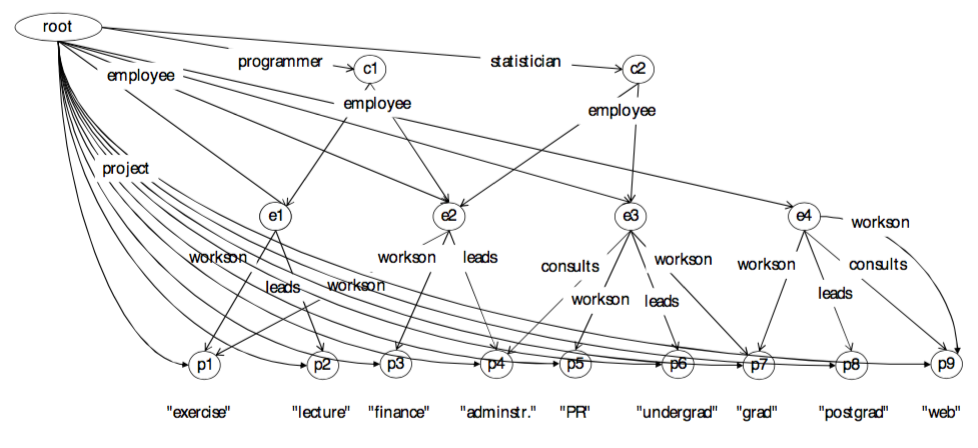
\includegraphics[width=\textwidth]{figures/data_graph.png}
\begin{itemize}
  \item Data graph: D = (V, E, R) is a labeled, rooted and directed graph. 
  \item V is a set of nodes
  \item E $\subseteq$ V x L x V is a set of labeled edges, they determine the meaning of the data values stored in the leaves
  \item R $\subseteq$ V is a set of root nodes that have no incoming edges. All nodes in V are reachable from some root in R
  \item A $\subseteq$ V are the atomic nodes = set of leaf nodes storing typed data values
  \item C $\subseteq$ A x U x T is the data stored in D, where U is the domain of all data values and T are the data types
\end{itemize}

\subsubsection{Structural Properties}
We can enumerate the paths starting from the root to capture the structure of the data graph. A possible schema would be to use a trie enumerating those paths and labeling the leaf nodes with the data type that is found in the graph database. However, it contains many redundant structures so it would be better to combine different subgraphs into a common graph structure. 

\subsubsection{Simulation and Schema Graphs}
Simulation is used to provide a criterion to decide whether a schema graph S correctly captures the structure of a data graph D. A schema graph may use alternate labels or wildcards on edges. Condition: for every node d in D reached by a path p starting from the root there exists a corresponding node s in S reachable by the same path and the types of the leaf nodes are the same in case d is a leaf node. S simulates D is denoted as D $<$ S.

More formal definition of the simulation relationship among labelled graphs:
\begin{itemize}
  \item Given graphs G$_{1}$, G$_{2}$ and relation R $\subseteq$ V$_{1}$ x V$_{2}$, then R is a simulation if for all labels l $\in$ L and for all x$_{1}$, y$_{1}$ $\in$ V$_{1}$ and for all x$_{2}$ $\in$ V$_{2}$ it holds that if x$_{1}$ $\rightarrow$$_{l}$ y$_{1}$ and R(x$_{1}$, x$_{2}$) then there exists y$_{2}$ $\in$ V$_{2}$ such that R(y$_{1}$, y$_{2}$) and x$_{2}$ $\rightarrow$$_{l}$ y$_{2}$
  \item If it holds, G$_{2}$ simulates G$_{1}$ and we can write G$_{1}$ $<$ G$_{2}$
\end{itemize}

We have to extend the concept of simulation relationship for the graph data model:
\begin{itemize}
  \item A schema graph S is a schema for a data graph D if there exists a rooted, typed simulation of D using S (that may contain wildcards and alternate labels). We require that root and leaf nodes in the data graph are related to root and leaf nodes in the schema graph. 
  \item Rooted simulation: R(r$_{1}$, r$_{2}$) for the roots r$_{1}$ and r$_{2}$  
  \item Typed simulation: for all x, y if R(x, y) and y is an atomic type then x must be an atomic node with content of that type
  \item For wildcards and alternate labels the label in the data graph has to be contained in the set of labels specified by these extended schema edge labels: if x$_{1}$ $\rightarrow$$_{l}$ y$_{1}$ then x$_{2}$ $\rightarrow$$_{l}$ y$_{2}$ or x$_{2}$ $\rightarrow$ $_{\_}$ y$_{2}$ or x$_{2}$ $\rightarrow$$_{l|k|...}$ y$_{2}$

\end{itemize}

\subsubsection{Classification by Schema Graphs}
We can define the rooted simulation R as a table with S nodes on the left (Class) and corresponding nodes in D on the right (Instances). The database schema classifies the data in the database.

\paragraph{Multiple classification}: a data node may belong to multiple classes. Two different valid simulations could classify the same data node in different classes (as it requires to be classified in at least one class, but not all possible classes), which could lead to ambiguous classification.

\paragraph{Maximal simulations}: it guarantees that the resulting classification is unique. Given two simulations R$_{1}$ and R$_{2}$ between a data graph and a schema graph the following holds: D $<$$_{R1}$ S and D $<$$_{R2}$ S then  D $<$$_{R1 \cup R2}$ S. The maximal simulation can be computed as a fixpoint iteration. 

\paragraph{Fixpoint iteration}: We start from the total relation between all nodes of D and S, i.e., data instances belong to all classes. Then we stepwise eliminate those pairs in R that violate the simulation condition. That is, whenever a pair should be contained in R we check whether a corresponding link exists in the data graph.
\begin{algorithm}
\caption{Fixpoint iteration for data graph D, schema graph S}
\begin{algorithmic} 
\STATE $R' \leftarrow \emptyset$
\STATE $R \leftarrow \{ (o, c) | o \in D, c \in S \}$
\WHILE{$R \neq R'$}
\STATE $R' \leftarrow R$
\STATE $R \leftarrow  \{ (o, c) |$ all $(o, c)$ such that either o is atomic value and c its type or there exists $(o', c') \in R'$ and $o \rightarrow _{l} o' \in D$ and $c \rightarrow _{l} c' \in S \}$
\ENDWHILE
\end{algorithmic}
\end{algorithm}

\subsubsection{Refining Schemas}
\begin{itemize}
\item Refinement is needed when a schema evolves and becomes more precise over time as more information on the databases become available. 
\item We say that schema S$_{1}$ subsumes schema S$_{2}$ if S$_{1}$ contains less detail and is more general than schema S$_{2}$. It implies that all databases that conform to S$_{2}$ also conform to S$_{1}$
\item This is the case if S$_{2}$ $<$ S$_{1}$. So if S$_{2}$ is a schema for D (D $<$ S$_{2}$) then we can conclude that D $<$ S$_{1}$ and therefore S$_{1}$ is also a schema for D.
\end{itemize}

\subsection{Schema Extraction}
The goal is to automatically construct a schema graph from the data graph. It should be:
\begin{itemize}
\item \textbf{Accurate}: every path that occurs in the schema graph occurs in the data graph and vice versa
\item \textbf{Concise}: every path occurs only once
\end{itemize}
It is called a \textbf{data guide}. Data guide nodes correspond to subsets of data graph nodes. Its root node is the set containing the data graph root. 
\subsubsection{Data Guide Construction}
For each data guide node constructed and for each edge label of an  edge leaving in the data graph some element from the data guide node:
\begin{itemize}
\item form the set of nodes in the data graph reached by this edge label
\item if the set exists already in the data guide, create a labeled edge to it
\item else create a new data guide node and connect it by the edge
\end{itemize}
Continue until no more new data guide nodes are created.
\\
\paragraph{Properties}
\begin{itemize}
\item Same nodes of data graph occur in multiple places $\rightarrow$ space complexity! Problem: node equivalence (if the paths leading to two nodes in the data graph are the same, the nodes are equivalent)
\item Repeating structures in the data graph are reduced to a single structure in the data guide (less edges)
\item Sometimes it can be more complex than the data graph itself
\item Deterministic graph = DFA. It is minimal, deterministic schema graph with 1:1  correspondence among data guide nodes and sets of nodes reached by the  same paths (strong dataguide)
\item Cycles in the data graph lead to cycles in the data guide
\end{itemize}
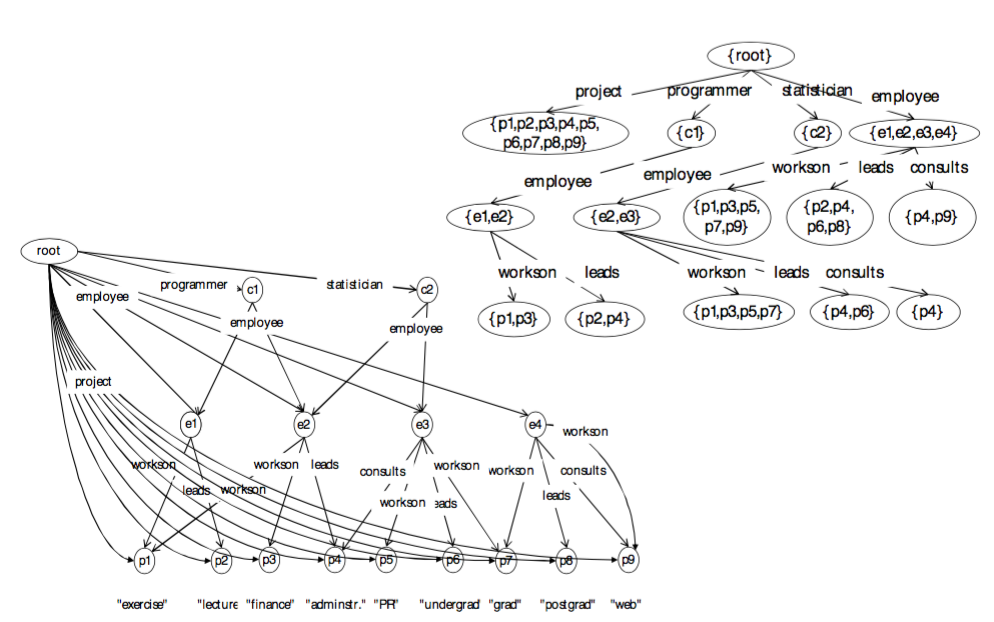
\includegraphics[width=\textwidth]{figures/data_guide.png}
\subsection{Schema Mapping}

